\section{Les applications}

L'un des principaux but du projet était de porter une application respectant 
certaines contraintes sur la carte présentée précédemment. En effet, la 
première contrainte était que le programme devait être capable de générer un 
trafic mémoire important sur le bus pendant une période de temps assez courte 
(environ une seconde). L'autre contrainte qu'il fallait respecter était que 
l'application devait pouvoir se trouver dans n'importe quelle voiture moderne. 
Ce sont ces deux raisons qui nous ont amené à choisir une application de calcul 
de plus court chemin basée sur des cartes OpenStreetMap. Ces cartes présentent
l'avantage d'être libres d'utilisation, gratuites et complètes. 

\subsection{Sélection de l'application}

L'application que nous avons décidé de porter sur la carte a été choisie selon 
un certain nombre de critères. \\

Tout d'abord, il fallait que celle-ci ne soit pas écrite en Java (comme c'est 
le cas pour de nombreuses applications utilisant les cartes OpenStreetMap) car 
le profilage mémoire aurait été dans ce cas plus difficile à effectuer à cause 
de la JVM. En effet, cette dernière effectue des optimisations au niveau de la 
mémoire qui nous aurait empêché de quantifier les besoins réels de 
l'application en terme de bande passante sur le bus. De plus, la quantité de 
mémoire disponible sur la carte étant relativement restreinte (1 Gio), nous ne 
pouvions pas nous permettre d'utiliser un language à ramasse-miettes comme 
Java sachant que les cartes OpenStreetMap sont elles aussi très gourmandes en 
mémoire. \\

Ensuite, un autre critère de sélection pour l'application fut le nombre de 
dépendances de la partie du programme s'occupant du calcul du plus court 
chemin. En effet, bien que ce ne soit pas gênant d'un point de vue des 
performances ou des accès mémoire, les dépendances rendent le portage de 
l'application plus complexe. Il était donc utile, dans la limite du possible, 
de trouver un programme avec un petit nombre de dépendences. \\

Enfin, le dernier critère de sélection fut le fait que l'application soit 
multi-threadé (ou qu'elle puisse l'être assez simplement). En effet, afin 
d'étudier l'impact de l'application sur la tâche temps réel, il faut pouvoir 
l'exécuter sur les trois coeurs du processeur qui ne sont pas occupés par la
tâche temps réel. Il aurait été possible de lancer trois instances d'un 
programme contenant un seul thread, mais cela ne nous a pas semblé réaliste 
vis-à-vis du scénario que nous considérons. En effet, dans une voiture moderne, 
l'application GPS n'est pas exécutée trois fois, mais elle contient plusieurs 
fils d'exécutions qui effectuent une partie du calcul. \\

En tenant compte des contraintes énoncées précédemment, nous avons trouvé deux
applications : Open Source Routing Machine (OSRM) et Routino. L'application que
nous avons porté sur la carte est Routino, pour des raisons qui seront énoncées
plus tard dans le rapport.

\subsection{Open Source Routing Machine}

Un des deux programmes que nous avons examiné de près est Open Source Routing 
Machine \cite{_open_????}. Cette application est une implantation 
très performante d'un moteur de calcul de plus court chemin en C++. 
Concrètement, c'est un serveur multi-threadé capable de gérer plusieurs calculs 
de chemins simultanément. Cependant, plusieurs raisons ont fait que nous 
n'avons pas choisi de porter cette application sur la carte. \\

Tout d'abord, le nombre de dépendences du programme est assez élevé (environ 
6 bibliothèques), ce qui rentre en contradiction avec ce qui a été dit 
précédemment et de ce fait rendait le portage de l'application inutilement
compliqué.\\
Ensuite, le programme qui effectue le calcul du plus court chemin est très 
gourmand en mémoire. En effet, les cartes OpenStreetMap sont assez volumineuses
($\sim$ 4.6 Gio pour la France compressée en bz2, et 22 Gio pour l'Europe). C'est
la raison pour laquelle toutes les applications possèdent un outil permettant 
de convertir ces cartes en un format plus léger et directement compréhensible 
par le programme qui va effectuer le calcul du plus court chemin. Cependant, 
dans le cas d'OSRM, cet outil ne produit pas des cartes assez légères, ce qui 
fait que le programme qui effectue le routage consomme environ 3 Gio de mémoire 
vive pour la carte de France. On ne peut donc pas utiliser ce programme avec la 
carte de France sur le système embarqué, car celui-ci ne contient qu'un Gio de 
mémoire vive, et on veut que le programme n'entraîne pas de swap. L'utilisation 
d'une carte plus petite (comme celle de l'Ile-de-France, par exemple) n'aurait 
pas aidé à régler le problème. En effet, comme le programme est très performant,
les temps d'exécutions sur la carte aurait été trop courts par rapport à ceux 
de la tâche temps réel.\\
Enfin, la façon dont l'application était parallélisée ne nous convenait pas. En 
effet, OSRM permet de lancer plusieurs calculs de plus court chemin en même 
temps mais l'algorithme effectuant ce calcul n'est pas lui-même parallèle. 
La parallélisation de cet algorithme nous a semblé peu pertinente au vu de la 
complexité de celui-ci et des inconvénients que nous avons vu précédemment.

\subsection{Routino}

L'autre application que nous avons étudié de manière approfondie est Routino 
\cite{bishop_routino_????}. C'est l'application que nous avons décidé de
porter sur la carte afin de pouvoir réaliser le profilage que nous verrons plus
tard.

\subsubsection{Présentation de l'application}

Routino est une application écrite en C qui permet de calculer le chemin le 
plus court (ou le chemin le plus rapide) entre deux points. Cette application 
n'étant pas multi-threadée, nous avons du effectuer le travail de
parallélisation, comme nous le verrons plus tard dans le rapport.

\paragraph{Raisons du choix de l'application}
Il existe plusieurs facteurs qui nous ont poussé à choisir cette application 
plutôt qu'une autre. D'une part, le nombre de dépendences du programme
effectuant le routage était nul, ce qui rendait le portage de l'application
trivial. En effet, il suffit de cross-compiler l'application avec un compilateur
ARM pour produire un exécutable compatible avec la carte. \\
D'autre part, l'outil permettant de convertir les données OpenStreetMap en 
fichiers compréhensibles par l'application effectuant le routage est assez 
efficace. En effet, pour la carte de France, les fichiers produits font environ 
860 Mio et peuvent donc rentrer sans problème dans la mémoire de la carte. Cela 
nous permet de calculer des plus courts chemins sur des distances plus 
conséquentes et donc d'augmenter le temps d'exécution de l'application.

\paragraph{Fonctionnement général de l'application}
Avant de pouvoir effectuer des calculs de plus court chemins, il faut dans un 
premier temps convertir les cartes OpenStreetMap en des fichiers compréhensibles
par l'application de routage. C'est le rôle de l'exécutable nommé
\texttt{planetsplitter}, qui produit les quatre fichiers suivants :

\begin{itemize}
\renewcommand{\labelitemi}{$\bullet$}
\item \texttt{nodes.mem} : C'est le fichier qui contient les noeuds du graphe.
\item \texttt{ways.mem} : C'est le fichier qui contient des informations 
relatives aux arcs du graphe (type de transport autorisé sur l'arc, ...).
\item \texttt{segments.mem} : C'est le fichier qui contient les arcs du graphe.
\item \texttt{relations.mem} : Fichier qui contient des informations sur les 
relations entre les arcs du graphe.
\end{itemize}

Une fois ces fichiers obtenus, on peut appeler le programme \texttt{router} qui 
est capable d'effectuer des calculs de plus court chemin entre deux points. 
Pour réaliser cette opération, le programme commence par mapper les fichiers 
vus ci-dessus en mémoire. Si on a découpé le trajet en plusieurs morceaux dans
l'appel à \texttt{router} (par exemple si on indique qu'on veut le chemin le 
plus rapide de Paris à Nice en passant par Pau), le programme va calculer 
séquentiellement les chemins les plus rapides bout par bout. Dans notre exemple,
cela veut dire que l'application va d'abord calculer le chemin le plus rapide de 
Paris à Pau, puis de Pau à Nice. Cela peut sembler évident, mais il est 
important d'avoir ceci à l'esprit lorsque l'on abordera la parallélisation de 
l'application. L'algorithme utilisé par l'application est l'algorithme A*. \\

Le fait que le programme mappe les fichiers produit par \texttt{planetsplitter} 
peut entraîner des résultats peu fiables lors de la réalisation des benchmarks
(seulement lors de la premiere exécution de Routino). En effet, lorsqu'un 
programme mappe des fichiers en mémoire, le système d'exploitation (ici Linux) 
peut ne pas remplir la mémoire avec ces fichiers, et attendre que l'application 
accède aux zones de mémoires concernées avant d'effectuer les entrées/sorties 
visant à rapatrier les fichiers en mémoire. De ce fait, lors de la première 
exécution du routeur, les temps d'exécution sont plus grands car les fichiers 
ne sont pas encore présents en mémoire. Cependant, lors des exécutions suivantes,
les temps sont plus faibles (et stables), car les données sont présentes dans le
cache du système. Il faut donc s'assurer de bien exécuter Routino une première 
fois avant de lancer les scripts de benchmarks (voir l'annexe \ref{ann:scripts}
pour plus d'informations). 
 
\paragraph{Utilisation de l'application}
L'utilisation des programmes \texttt{planetsplitter}, \texttt{router} et 
\texttt{router\_multi} est expliquée en détail dans l'annexe \ref{ann:routino}.

\subsubsection{Parallélisation}
\paragraph{Première approche}
Notre première intention fut de paralléliser l'algorithme effectuant le parcours
de plus court chemin. Cependant, après examen du code, nous sommes arrivés 
à la conclusion que l'implantation présente dans le programme est difficilement
parallélisable. En effet, l'algorithme utilise systématiquement les valeurs 
des itérations précédentes pour effectuer son calcul.

\paragraph{Seconde approche}
Plutôt que de paralléliser en profondeur l'algorithme, on se fixe l'objectif de
paralléliser le calcul des segments passés en paramètre de l'itinéraire. Ainsi,
si l'on souhaite calculer un itinéraire pour se rendre de Paris à Nice en
passant par Pau, on calculera en même temps Paris-Pau et Pau-Nice. Cette
approche permet de rendre multi-tâches l'application rapidement et avec un
minimum de données partagées entre les tâches, puisque les calculs de portions
sont indépendants les uns des autres. La version multithread de Routino propose
donc une option \texttt{--threads} afin de spécifier le nombre de tâches 
s'exécutant pour calculer l'itinéraire. Nous proposons l'implantation suivante :
\begin{itemize}
\renewcommand{\labelitemi}{$\bullet$}
\item la tâche principale (\texttt{main}) analyse les options et prépare les
  données pour le calcul de chaque portion. Elle lance ensuite le nombre de
  tâches demandées, calcule la dernière portion, puis s'endore en attendant que
  toutes les portions soient calculées. Elle se réveille ensuite pour rassembler
  les résultats et produire les fichiers de sortie.
\item les tâches filles piochent dans la liste des portions à calculer et
  calculent l'itinéraire associé à la portion. Lorsqu'il n'y a plus de portion
  à calculer, la tâche meurt. Si elle était la dernière tâche fille, elle
  débloque la tâche principale avant de mourir.
\end{itemize}
\paragraph{}
Pour vérifier que la parallélisation était efficace, nous avons mesuré à l'aide
des scripts \texttt{cpusage.sh}, \texttt{threadusage.pl} et \texttt{speedup.sh}
(Annexes \ref{ann:cpusage} et \ref{ann:speedup})
respectivement l'utilisation globale des coeurs du processeur, l'utilisation du
processeur par chaque tâche et le temps d'exécution en comparaison avec la 
version monothread de Routino (Figures \ref{fig:cpusage}, \ref{fig:threadusage}
et \ref{fig:speedup}).

\begin{figure}[H]
\centering
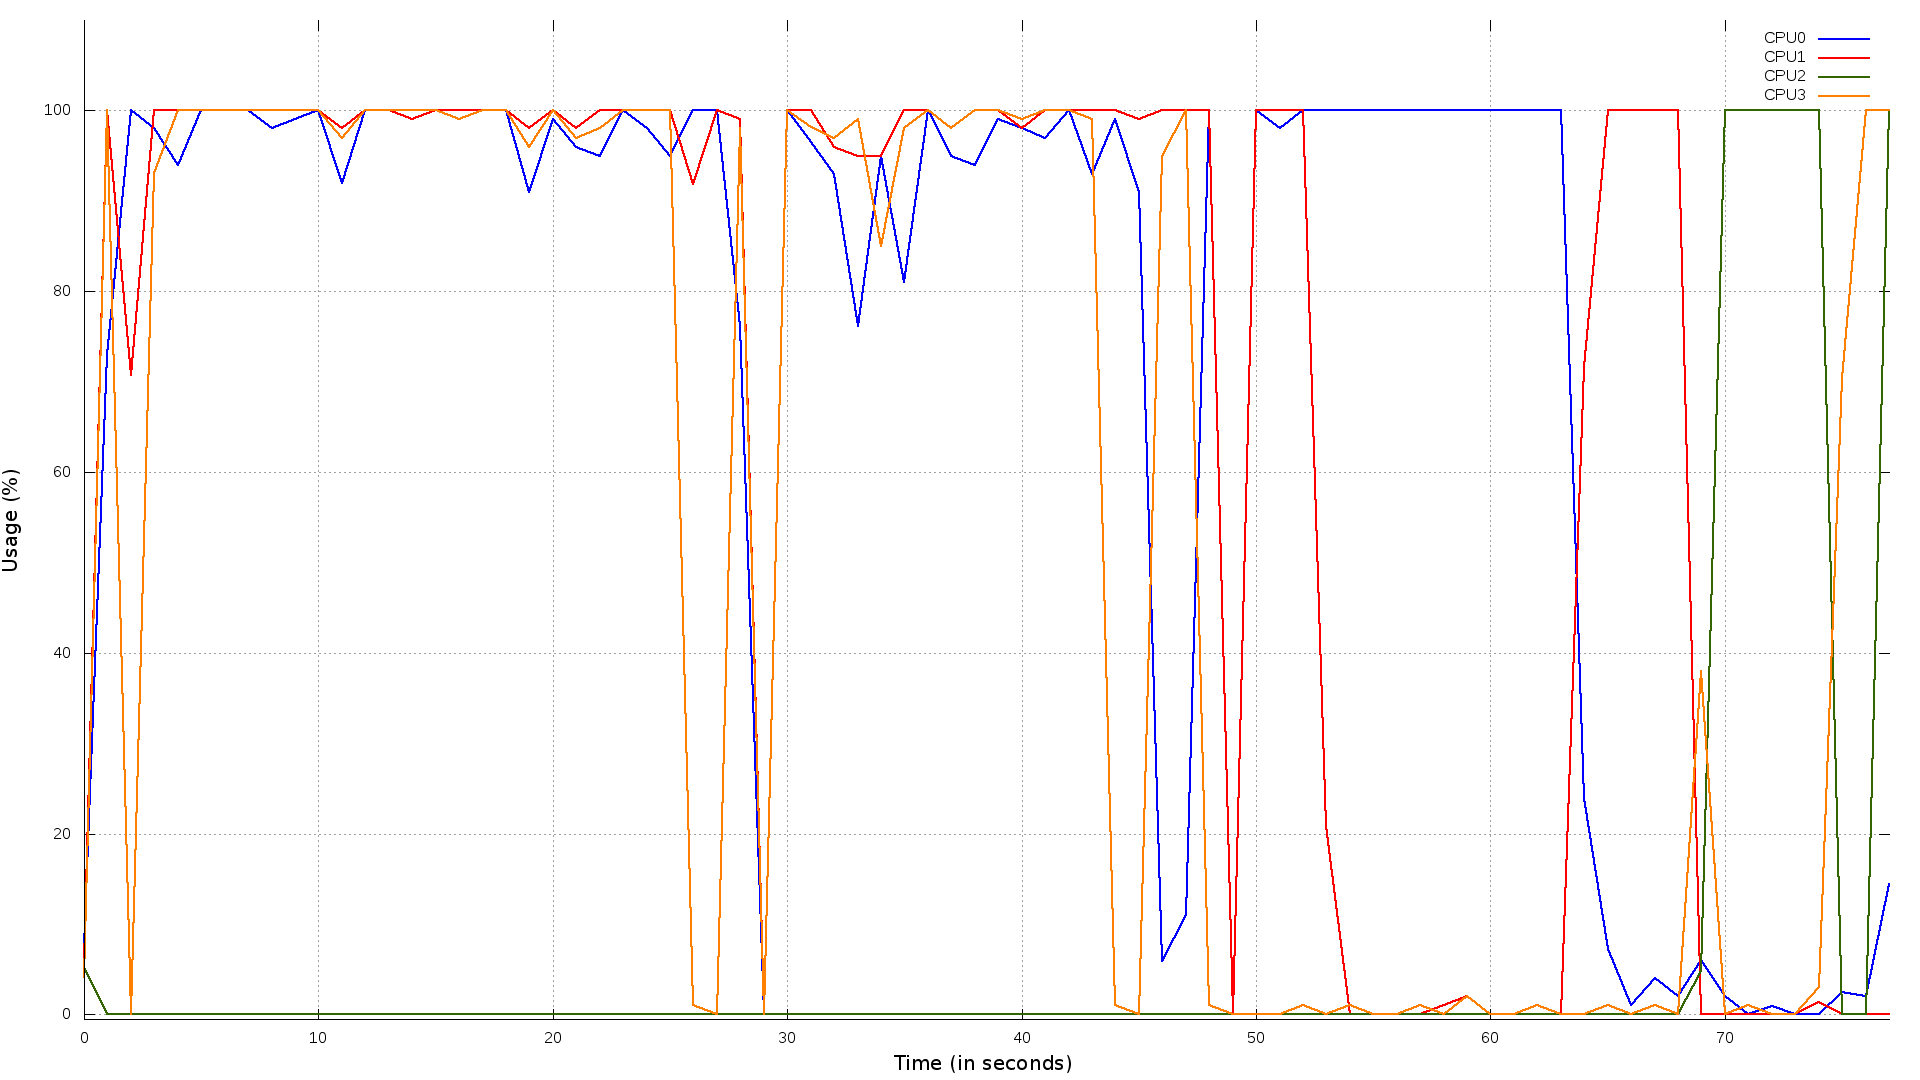
\includegraphics[scale=0.285]{include/cpu_usage.png}
\caption{Utilisation CPU par coeur lors de l'exécution de Routino multithread}
\label{fig:cpusage}
\end{figure}

\paragraph{}
Sur la figure \ref{fig:cpusage}, on observe bien que trois coeurs tournent à
100\% la majorité du temps, et que le quatrième n'est pas utilisé. Cela montre
que l'application utilise bien trois threads comme prévu, sachant qu'elle tourne
seule sur la machine. L'activité diminue sur la fin de l'exécution car certaines
portions de l'itinéraire sont plus courtes à calculer que d'autres.\\
La figure \ref{fig:threadusage} nous montre l'activité de chaque thread de
l'application. On constate une forte activité en début d'exécution sur les trois
threads, chacun calculant des portions d'itinéraire. On remarque la terminaison
de chacune des tâches tour à tour, n'ayant plus de portion à calculer, ainsi
que le réveil de la tâche \texttt{main} pour mettre enf orme les résultats.\\
De plus, on remarque un gain de performances (Figure \ref{fig:speedup}) de la 
version multi-thread (ci-après appelé Routino MT) par rapport à la version
monothreadée de Routino.

\begin{figure}[H]
\centering
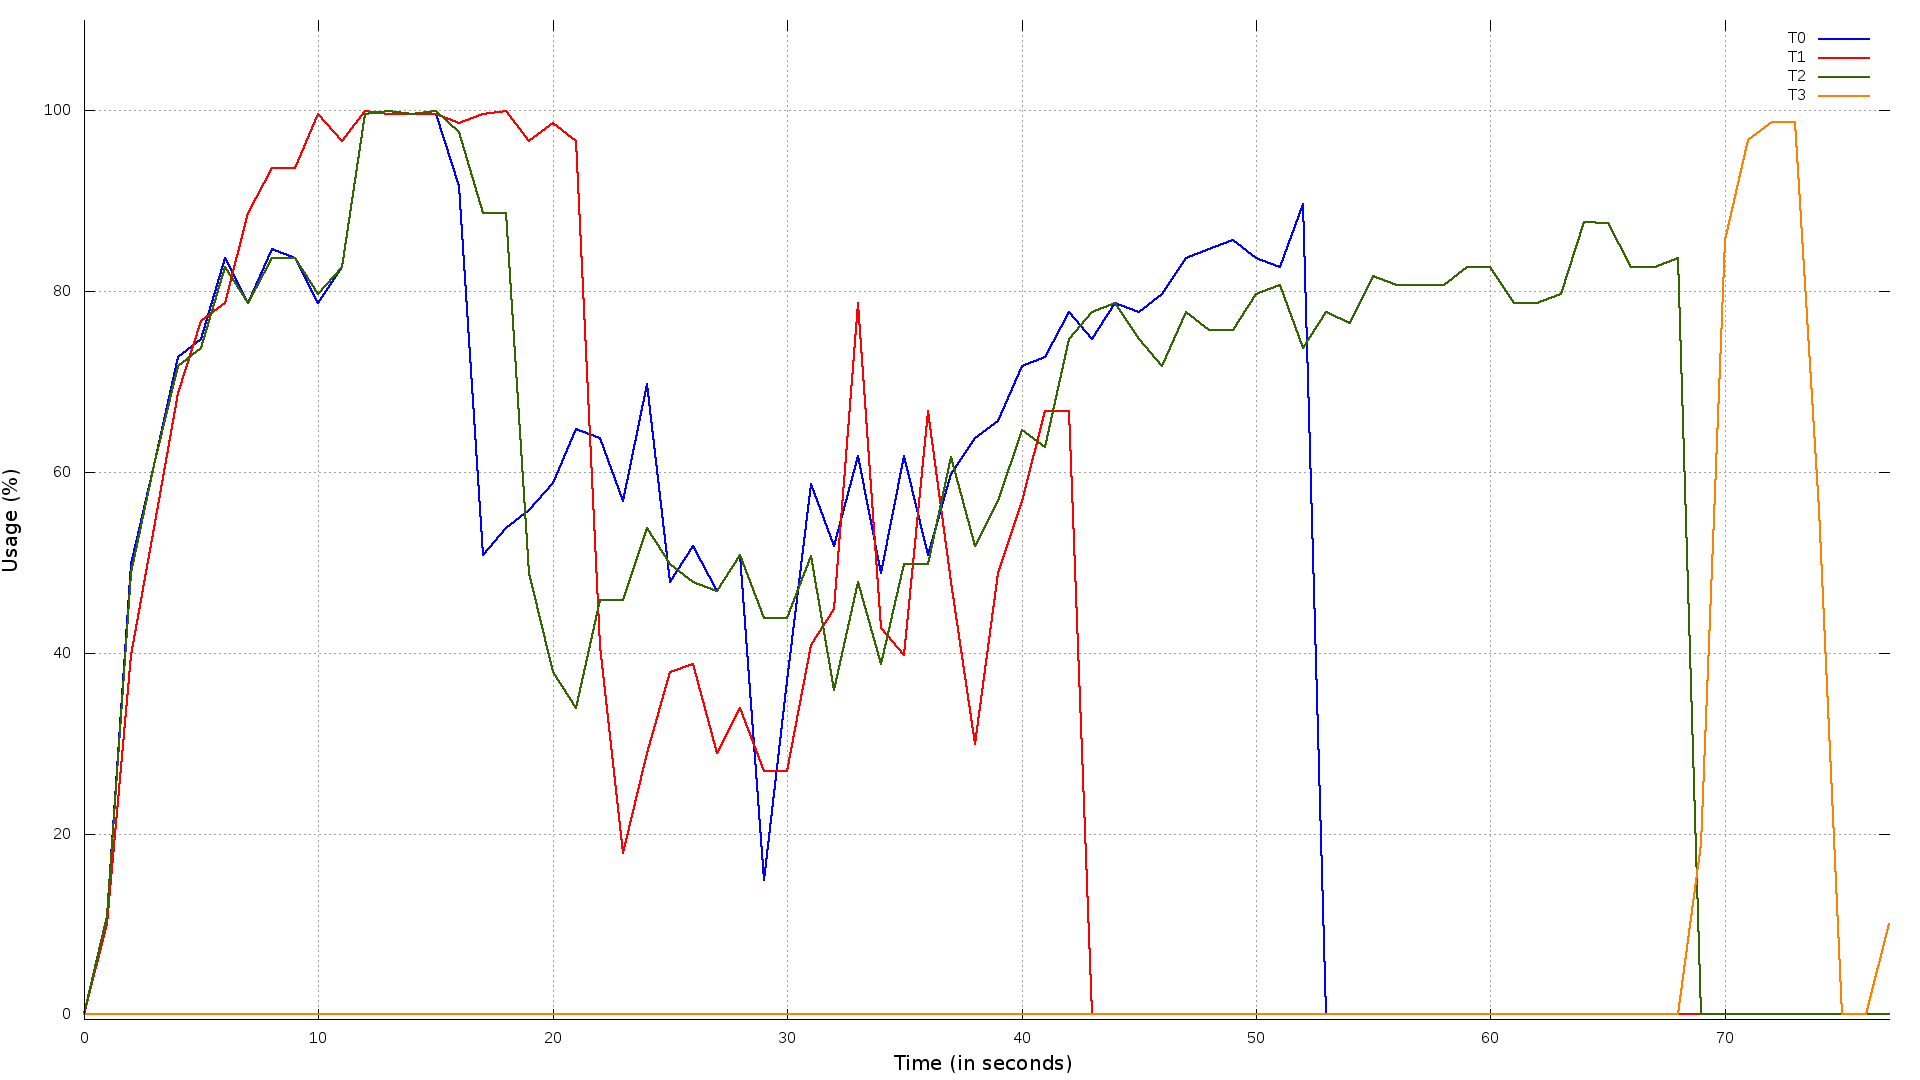
\includegraphics[scale=0.27]{include/thread_usage.png}
\caption{Utilisation CPU par tâche lors de l'exécution de Routino multithread}
\label{fig:threadusage}
\end{figure}

\begin{figure}[H]
\centering
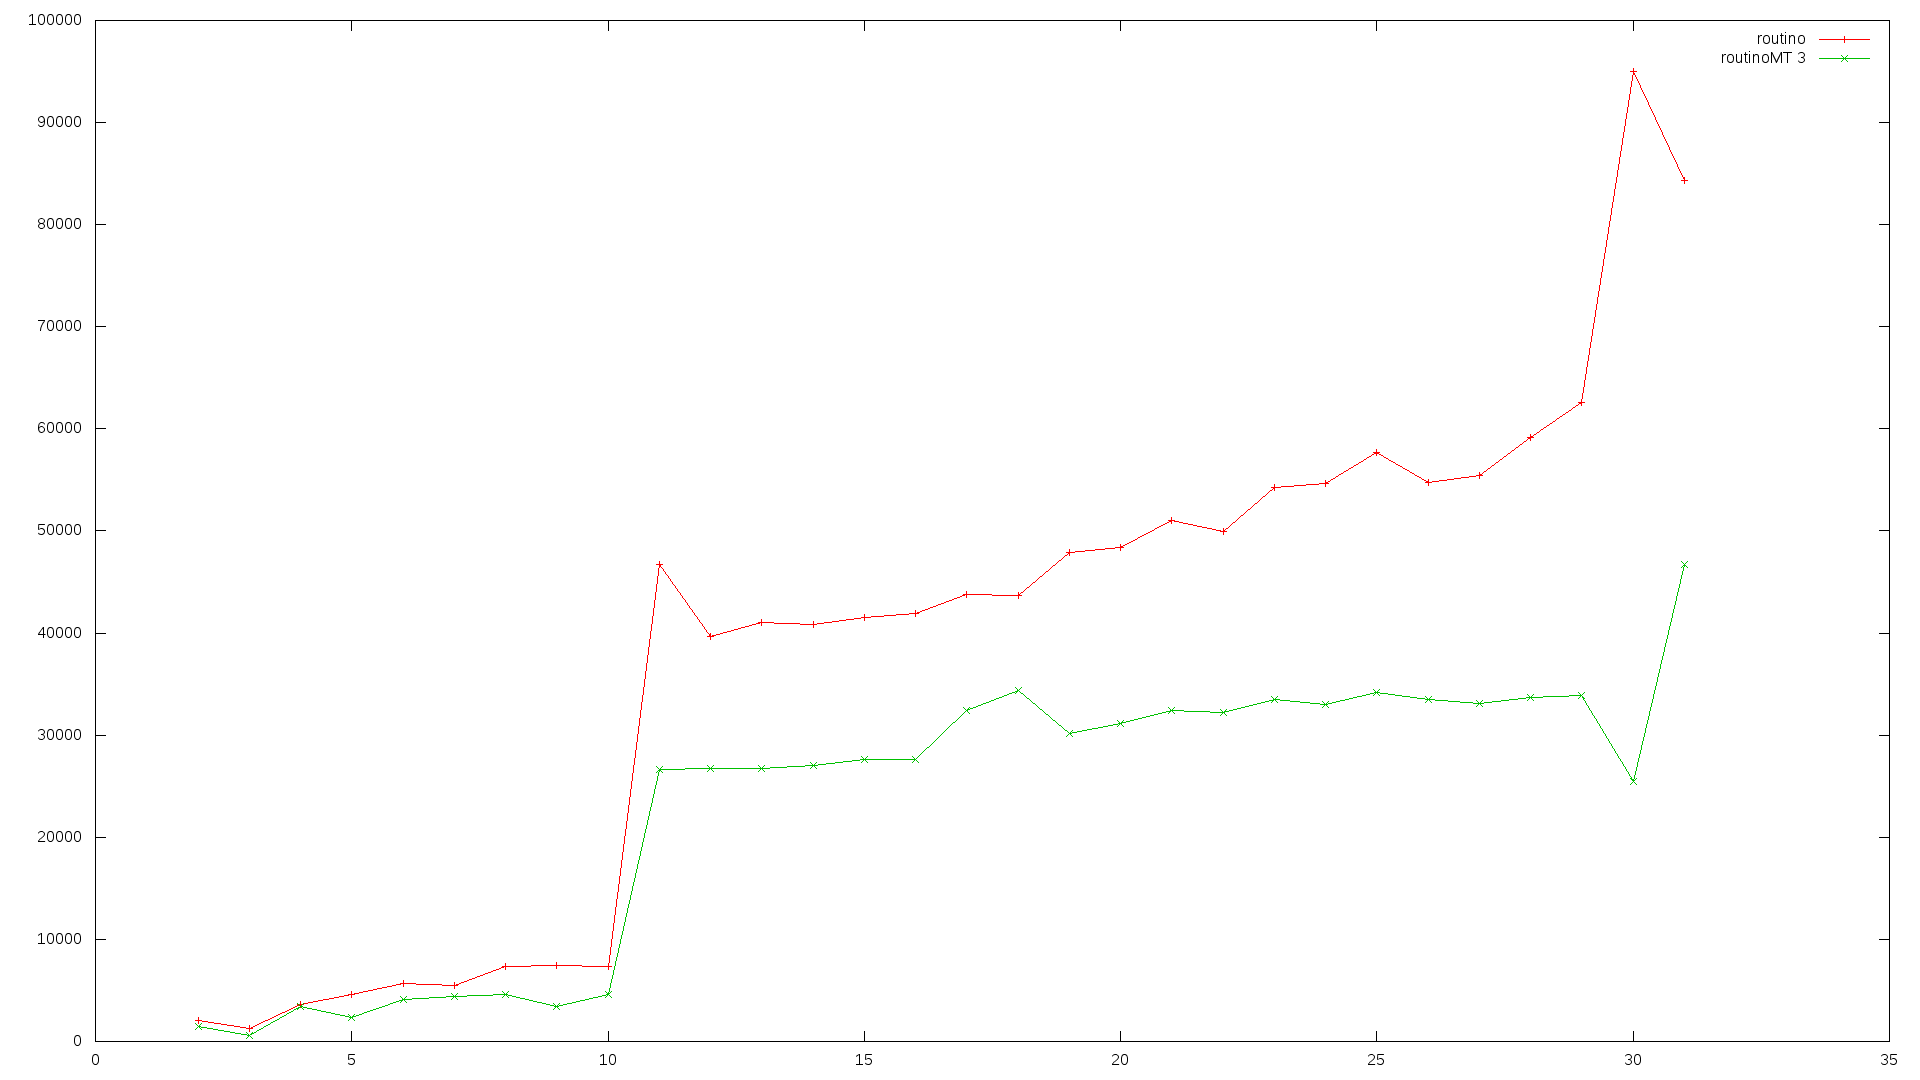
\includegraphics[scale=0.27]{include/speedup.png}
\caption{Temps d'exécution de Routino (en rouge) et de Routino MT (en vert) par
rapport au nombre de portions}
\label{fig:speedup}
\end{figure}

\subsection{Les tâches temps réel}

Les tâches temps réel que nous avons utilisé lors de notre projet sont issues 
de la suite logicielle \texttt{MiBench} \cite{guthaus_mibench:_2001}. Les 
programmes dont nous nous sommes servis sont les suivants : 

\begin{itemize}
\renewcommand{\labelitemi}{$\bullet$}
\item \texttt{qsort} : Cette tâche effectue un quicksort sur le fichier qui lui 
est donné en entrée. Dans notre cas, le fichier contient un ensemble de nombres.
\item \texttt{susan} : Cette tâche est un programme de reconnaissance d'images 
capable de reconnaitre les coins et les bordures. Nous utilisons le programme 
avec le grand jeu de donnée fourni avec la suite MiBench (une image complexe 
en noir et blanc).
\item \texttt{patricia} : Les Patricia tries sont des arbres préfixes obtenus 
en fusionnant chaque noeuds n'ayant qu'un fils avec celui-ci. Cette structure 
est particulièrement adaptée pour la recherche d'éléments. Ce programme effectue
des ajouts et des recherches dans des Patricia tries. Le jeu de données que
nous utilisons est un ensemble d'adresses IP ayant effectué des requêtes sur un
serveur web assez fréquenté.
\item \texttt{aes} : Programme qui effectue un cryptage/décryptage de données 
avec AES. Le jeu de donnée utilisé en entrée est un texte ASCII trouvé en ligne.
\item \texttt{fft} : Programme qui effectue une transformée de Fourier rapide (et 
son inverse). 
\end{itemize}
